% This is samplepaper.tex, a sample chapter demonstrating the
% LLNCS macro package for Springer Computer Science proceedings;
% Version 2.20 of 2017/10/04
%
\documentclass[runningheads]{llncs}
%
\usepackage{graphicx}
%% Language and font encodings
\usepackage[portuges]{babel}
\usepackage[T1]{fontenc}
\usepackage{verbatim}

\setcounter{secnumdepth}{6}
\renewcommand\theparagraph{\Alph{paragraph}}
 
\makeatletter
\renewcommand\paragraph{\@startsection{paragraph}{4}{\z@}%
                                      {-3.25ex\@plus -1ex \@minus -.2ex}%
                                      {0.0001pt \@plus .2ex}%
                                      {\normalfont\normalsize\bfseries}}
\renewcommand\subparagraph{\@startsection{subparagraph}{5}{\z@}%
                                      {-3.25ex\@plus -1ex \@minus -.2ex}%
                                      {0.0001pt \@plus .2ex}%
                                      {\normalfont\normalsize\bfseries}}
 
\counterwithin{paragraph}{subsubsection}
\counterwithin{subparagraph}{paragraph}
\makeatother
 
% Used for displaying a sample figure. If possible, figure files should
% be included in EPS format.
%
% If you use the hyperref package, please uncomment the following line
% to display URLs in blue roman font according to Springer's eBook style:
% \renewcommand\UrlFont{\color{blue}\rmfamily}

\begin{document}
%
\title{Sistemas de Recomendação: Introdução e Aplicações Comerciais\thanks{Supported by organization x.}}
%
%\titlerunning{Abbreviated paper title}
% If the paper title is too long for the running head, you can set
% an abbreviated paper title here
%
%\author{First Author\inst{1}\orcidID{0000-1111-2222-3333} \and
%Second Author\inst{2,3}\orcidID{1111-2222-3333-4444} \and
%Third Author\inst{3}\orcidID{2222--3333-4444-5555}}
%
\authorrunning{F. Author et al.}
% First names are abbreviated in the running head.
% If there are more than two authors, 'et al.' is used.
%
\institute{Universidade do Minho, Gualtar, Portugal}
%
% typeset the header of the contribution
%
\begin{abstract}
The abstract should briefly summarize the contents of the paper in
150--250 words.

\keywords{Sistemas de Recomendação  \and Second keyword \and Another keyword.}
\end{abstract}
%
%
%

% Aqui começam os capitulos abordados pelo trabalho

\section{Definição e História}

\par Há cerca de 25 anos a internet tornou-se extremamente popular nos países desenvolvidos. Nos Estados Unidos da América, entre 1994 e 2000, observou-se um período de crescimento exponencial no uso e adoção da internet conhecido como a bolha da internet (em inglês, dot-com bubble). Empresas de todos os domínios tiveram que se adaptar a este facto e moveram os seus negócios online. 

\par As recomendações são uma parte crucial da experiência digital personalizada ao utilizador por qualquer empresa. Um utilizador passa, em média, entre seis a oito horas por dia online ~\cite{ref_history1}, gerando dados relativos á sua atividade. 

\par Surgiu, então, a idade de utilizar estes na recomendação de produtos. 

\par Devido ao sucesso obtido na sua implementação, os sistemas de recomendação mantiveram-se populares desde então e têm vindo a ser refinados. A Amazon, por exemplo, estima que 35\% das suas vendas são provenientes do uso de sistemas de recomendação~\cite{ref_history2}. 

\par Sistemas de recomendação de alta qualidade podem transformar a experiência do utilizador agradável e estabelecer confiança e lealdade a longo termo. 

\par Os sistemas de recomendação evoluíram de gerarem simples colunas de itens ou artigos a construir páginas dinâmicas que amplificam diversos objetivos provenientes da análise do comportamento e histórico do utilizador. 

\section{Técnicas utilizadas por sistemas de recomendação}

\begin{center}
\normalsize{\bfseries Modelos básicos dos sistemas de recomendação}\hfill
\end{center}


\par Os modelos básicos para sistemas de recomendação utilizam dois tipos de dados: interações utilizador-item como avaliações ou hábitos de compras e informações de atributos sobre utilizadores e itens como o perfil respetivo~\cite{ref_book1}. Os métodos que usam o primeiro tipo de dados referido são chamados de Métodos de filtragem colaborativa, enquanto os restantes que utilizam o segundo dão pelo nome de Métodos de recomendação baseados em conteúdo~\cite{ref_book1}.
\par Os métodos de recomendação baseados em conteúdo na maioria dos casos também fazem uso de matrizes de avaliações embora se foquem nas de um utilizador em vez de nas de um grupo de utilizadores~\cite{ref_book1}.
\par Em Sistemas baseados em conhecimento as recomendações não são baseadas em histórico de compras ou avaliações, em vez disso usam conhecimento sobre os requerimentos do utilizador~\cite{ref_book1}.
\par Alguns sistemas de recomendação combinam estes aspetos para criar sistemas híbridos. Estes sistemas combinam as forças dos vários tipos de sistemas para ter uma boa performance independentemente dos dados disponíveis~\cite{ref_book1}.
\hfill

\subsection{Sistemas de filtros colaborativos}

\hfill

\par Modelos de filtragem colaborativa usam avaliações de vários utilizadores para fazer recomendações.

\par O principal desafio para estes modelos reside nas matrizes esparsas.

\par Por exemplo, numa plataforma de música como o spotify, em que as músicas têm maior cotação dependendo do número de vezes que são ouvidas por um utilizador e em que os utilizadores só ouviram algumas das músicas disponíveis, as matrizes Utilizador x Música têm poucas avaliações visto que uma grande parte das músicas não foram ouvidas ainda.

\par Nestes modelos as avaliações não existentes podem servir como input. Por exemplo se dois utilizadores, Alice e Bob, em muitas músicas têm classificações parecidas, o algoritmo pode estabelecer uma relação de semelhança entre eles. Desta forma o algoritmo pode prever que em músicas nas quais só um tenha dado classificação, o outro terá uma apreciação parecida. Esta forma de previsão consegue colmatar uma parte das classificações inexistentes na matriz.







\hfill

\subsubsection{ Filtros Colaborativos Baseados em Utilizadores}

\hfill

 \par Neste caso as classificações fornecidas por utilizadores com os mesmos gostos de A são usadas para as recomendações para A. 

 \par A ideia básica destes tipo de filtros passa por encontrar utilizadores com gostos semelhantes a A através das semelhanças entre classificações dadas por estes nas mesmas músicas. Desta forma se B tiver os mesmos gostos de A e se B der uma boa classificação a uma música C é provável que A também dê uma avaliação positiva à mesma música. Ao conjunto de utilizadores usados para inferir essas previsões dá-se o nome de vizinhança.

\newline

\hfill

\begin{figure}[H]

  \centering

  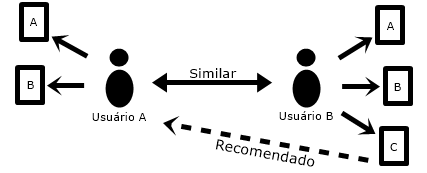
\includegraphics[scale = 0.35]{filtroutilizadoressimilares.png}

  \caption {Filtro Baseado em Utilizadores Similares}

  \label {fig01}

\end{figure}



\subsubsection{ Filtros Colaborativos Baseados em itens}

\hfill

 \par Para fazer previsões sobre se um utilizador A gostará de uma música B , o primeiro passo passa por determinar as X músicas mais semelhantes a B. As avaliações dadas por A a essas X músicas é usada para inferir se A gostará da música B.

 \par Este método é fácil de implementar, no entanto peca por falta de personalização.~\cite{ref_article1}.\newline

\begin{figure}[H]

  \centering

  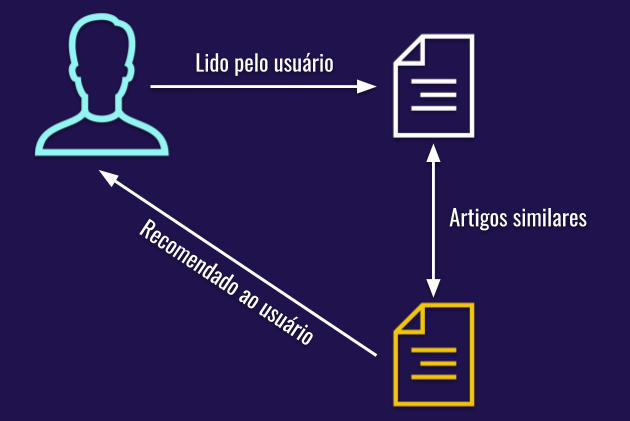
\includegraphics[scale = 0.2]{filtroitenssimilares.png}

  \caption{Filtro Baseado em itens Similares}

  \label{fig02}

\end{figure}
\par A vizinhança para estes métodos pode ser definida de duas formas:



\begin{center}
\normalsize{\bfseries Métodos Baseados em Memória}\hfill
\end{center}

 \par Estes métodos são também conhecidos como algoritmos de filtros colaborativos de vizinhança. Nestes, as avaliações que um utilizador pode dar a certos itens é prevista com base na sua vizinhança.\newline

\textbf{Vantagens:}\hfill
\hfill
\par 1. Simples de implementar e as recomendações feitas são facilmente explicáveis.\newline

\textbf{Desvantagens:}\hfill
\hfill
\par 1. Não funcionam bem com matrizes de avaliações esparsas, podendo não haver classificações suficientes para garantir que A goste da recomendação feita.\newline

\begin{center}
\normalsize{\bfseries Métodos Baseados em Modelos}\hfill
\end{center}
\hfill
\par Nestes modelos, mineração de dados e aprendizagem máquina são usados no contexto de modelos de previsão.
\par Nos casos onde o modelo é parametrizado, os parâmetros são aprendidos dentro do contexto da otimização da "framework".





\hfill
\subsection{Sistemas de Recomendação Baseados em Conteúdo}
\hfill
\par Nestes sistemas, os atributos descritivos dos itens são usados para fazer recomendações. O termo conteúdo refere-se as decrições dos itens. 
\par As classificações do utilizador, bem como os seus hábitos de compras são combinados com os atributos dos itens para fazer as recomendações. 
\par Por exemplo, num filme X o João atribuiu uma classificação elevada mas não temos acesso a mais nenhuma classificação do mesmo filme feita por outros utilizadores. Nestas situações Modelos de filtros colaborativos não servem. No entanto, a descrição do filme contém as mesmas palavras chave que outros filmes, logo estes podem ser sugeridos ao João.
\par Em métodos baseados em conteúdo as descrições dos itens, que estão marcadas com classificações são usadas para treino para criar sugestões especificas para o utilizador. Para cada utilizador os dados usados para treino do sistema de recomendação passam pelo histórico de compras e classificações.\newline


\begin{figure}[H]
  \centering
    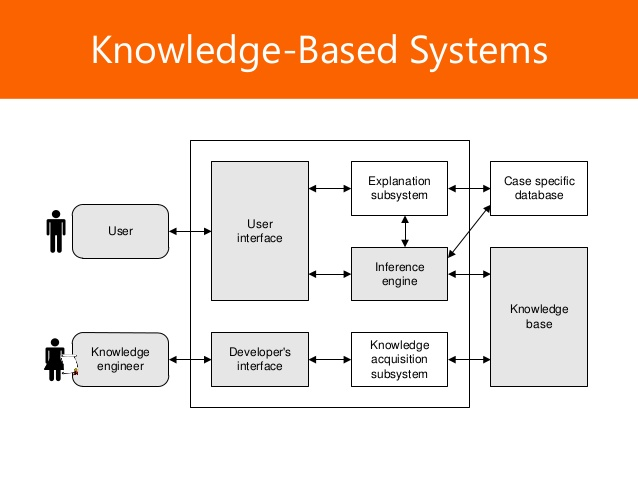
\includegraphics[scale = 0.3]{knoledgebasedsistems.jpeg}
    \caption{Sistema de Recomendação Baseado em Conteúdo}
    \label{fig03}
\end{figure}

\textbf{Vantagens:}\hfill
\hfill
\par 1. Quando não existem dados suficientes sobre um item, podemos inferir a futura experiência do utilizador usando as descrições do produto e comparando-as com os produtos sobre os quais o utilizador já se pronunciou. Desta forma o sistema pode contornar a falta de dados sobre as escassas clasificações de um item.\newline
\hfill
\par 2. O utilizador novo pode especificar palavras chave no seu perfil para serem feitas recomendações com estes modelos, isto é útil em cenários "cold-start".\newline

\textbf{Desvantagens:}\hfill
\hfill
\par 1. Caso o utilizador não tenha visto um determinado tipo de itens ainda que goste dele estes não serão recomendados, reduzindo a diversidade dos itens recomendados.\newline
\hfill
\par 2. Não são indicados para recomendações a novos utilizadores, visto que não há um histórico com o qual se pode treinar o sistema, uma vez que para ter um SR robusto é necessário ter um histórico.\newline


\subsection{Sistemas de Recomendação Baseados em Conhecimento}
\hfill
\par Estes sistemas são particularmente úteis em casos em que não há histórico de compras ou avaliações, ou cenários de cold-start.
\par Para além disso a natureza das preferências de um utilizador pode evoluir com o tempo. Como estes modelos utilizam as preferências dos itens conseguem acompanhar a tendência.
\par Em outros casos pode ser dificil acompanhar as preferências de um utilizador se este apenas estiver interessado num atributo específico do item.
\par O processo de escolha de recomendações baseia-se na similaridade entre requerimentos do utilizador e descrição dos itens, isto permite maior controlo do utilizador sobre o processo de recomendação podendo este explicitar o que pretende.
\par Estes sistemas podem ser classificados com base no tipo de interface: 
\hfill


\subsubsection{Sistemas de recomendação baseados em restrições}
\hfill
\newline
\par Utilizador especifica os atributos que pretende obter nos itens que procura. Regras especificas do dominio em que se insere a busca são utilizadas. Estas regras representam o conhecimento do sistema. Outras regras podem ser restrições no que diz respeito ao utilizador, por exemplo investidores experientes não fazem investimentos de alto risco. 
\par Posteriormente a uma pesquisa, o utilizador pode modificar os requisitos originais. Este processo é iterativo até o utilizador estar satisfeito com os resultados.
\hfill


\subsubsection{Sistemas de recomendação baseados em casos}
\hfill
\newline
\par Neste tipo de sistemas, o utilizador especifica casos em vez de preferências como pontos de referência. As métricas de semelhança são cuidadosamente definidas no contexto do dominio em que se inserem, formando assim a base de conhecimento do sistema. Os resultados obtidos são comummente usados como referências para novas pesquisas do utilizador. Por exemplo, caso um resultado de pesquisa se assemelhe ao que o utilizador pretende, este pode selecionar esse resultado preferêncial juntamente com alguns requerimentos extra na próxima pesquisa. Este processo guia o utilizador até ao item pretendido.
\par O sistema fornece sempre a oportunidade ao utilizador para mudar os requerimentos. No primeiro caso, as regras são usadas para guiar a busca com base nas similaridades com outros artigos. Já nos sistemas baseados em casos, o objeto de referência fornecido pelo utilizador é utilizado para calcular a similaridade com outros itens.
\par Os sistemas baseados em conhecimento partilham algumas das desvantagens
dos sistemas baseados em conteúdos, tendo como exemplo a falha de apresentar novo conteúdo que o utilizador não requisite, mas possa gostar. Para além disso, este sistema não aprende com o comportamento passado do utilizador, mas depende apenas dos requisitos que este inserir na pesquisa.
\hfill


\subsubsection{Sistemas de recomendação baseados em utilidade}
\hfill
\newline
\par Sistemas que fazem uso de funções de utilidade para computar a probabilidade de um utilizador gostar do item em questão.
O desafio ao aplicar estes métodos reside em definir a função apropriada para o utilizador visado. Estas funções podem ser vistas como conhecimento externo, resultando na contemplação dos sistemas como casos especificos de sistemas de recomendação baseados em conhecimento, partilhando assim das suas vantagens e desvantagens.
\hfill

\subsection{Sistemas de Recomendação Demográficos}\hfill
\par Nestas técnicas a localização do utilizador alvo é utilizada para saber a tendência de uma pessoa a comprar determinado produto. Por exemplo, nas zonas do país em que água é mais calcária que o normal, a tendência é de comprar detergentes que previnam o acúmulo deste mineral nas máquinas de lavar roupa.Em muitos casos, as informações demográficas podem ser combinadas com o contexto atual de informação do utilizador para guiar o proceso de recomendação.
\par Embora estes sistemas por si só não forneçam as melhores recomendações, combinados com outros sistemas produzem resultados significativamente melhores.
\hfill
\subsection{Sistemas de Recomendação hibridos/Agregados}
\hfill
 \par Nos três principais sistemas de recomendação descritos anteriormente, podemos observar que estes funcionam bem em cenários diferentes. 
 \par Os sistemas com filtros colaborativos dependem das avaliações da comunidade, métodos baseados em conteúdos dependem das descrições dos itens e avaliações do utilizador a quem a recomendação é feita e os sistemas baseados em conhecimento depende das interações sistema utilizador. Similarmente sistemas demográficos usam perfis demográficos para fazer recomendações.
 \par Como podemos observar cada uma das técnicas tem as suas vantagens e desvantagens, algumas funcionam melhor com cold-start e outras quando já têm uma base sólida de avaliações do utilizador. Isto leva-nos a concluir que, conjugando os vários sistemas, conseguimos construir algoritmos mais robustos e com melhor performance. Usualmente existe uma grande variedade de inputs o que nos dá a flexibilidade para empregar uma grande variedade de técnicas na mesma tarefa.
 \par Os sistemas híbridos estão extremamente relacionados com os campos da análise de conjuntos nos quais o poder de múltiplos tipos de algoritmo de aprendizagem máquina é combinado para criar um modelo mais robusto.
 \par Sistemas de recomendação agregados são capazes de combinar não só o poder de múltiplas fontes de dados como também ser altamente eficazes ao combinar múltiplos modelos num só tipo. Este cenário não é muito diferente da análise de conjuntos no campo de classificação de dados.


\section{Vantagens para o promotor de recomendação}
\section{Vantagens para o alvo da recomendação}
\section{Algoritmos de Machine Learing Utilizados}
\section{Exemplos caraterísticos}
\subsection{ Serviços de Filmes: NetFlix}
\hfill
\par O modelo de negócio da NetFlix consiste num serviço de subscrição que oferece recomendações personalizadas, para ajudar os clientes a encontrar as séries e filmes que lhes interessam.
\par O SR da Netflix consiste num conjunto de vários algoritmos, que servem para diferentes casos e se fundem para criar uma “experiência completa” na plataforma.
\par Neste caso, os algoritmos para os sistemas de recomendação trabalham com o padrão standard $input> predição> resultado$. Como atributos de input temos: classificação, título do filme e número de estrelas que são atribuídas pelos utilizadores. As previsões de $ratings$ são calculadas com base nas informações que já existem no sistema, usando um sistema RMSE ($Root$ $Mean$ $Squared$ $Error$) onde é possível escolher quais os valores dos dados já existentes e dos dados que ainda não existem, criando assim uma recomendação \cite{ref_url1}.
\par O sistema de recomendação da Netflix é dividido em dois sistemas de organização e monitorização: o das $Metatags$ e o Comportamento do utilizador na plataforma. 
\par Tudo começa com a organização do catálogo da Netflix em categorias, subcategorias, géneros e tipos, todos sugeridos por um sistema de $tags$ abrangente e preciso. Para tal, a plataforma adopta as $metatags$, que são etiquetas que classificam todos os conteúdos disponíveis. Isto é, as metatags contêm informações que analisam cada característica dos títulos, tais como: o ano de produção, prémios, actores, directores, entre outras características. 
\par Como atributos para os algoritmos do SR da Netflix também podemos considerar as avaliações, comentários gerados pelos assinantes e até o comportamento do assinante na plataforma. Esta supervisão do comportamento do utilizador na interface do serviço abrange informações como: o tempo que o utilizador ficou em cada sector da plataforma, o tipo de dispositivo onde está a visualizar os conteúdos. Posteriormente, todas estas informações são cruzadas, gerando as recomendações personalizadas para cada um dos utilizadores. Segundo a Netflix três a cada quatro vídeos assistidos no sistema só foram visualizados porque estavam na lista de recomendações. Atualmente a NetFlix tem investido no uso de redes neuronais.






\subsection{ Serviços de Músicas: Spotify}

\par A Música é essencial, como a comida, por exemplo, no entanto o tipo da comida varia de acordo com o nosso estado mental. A maneira como respondemos a estímulos, independentemente de cada um deles, é estritamente pessoal e com os sons isso não é diferente. Tendemos a ouvir canções mais animadas quando estamos mais alegres e do mesmo modo preferimos as tristes quando estamos em dias maus.
\par Um observador pode prever o estado emocional  de um utilizador apenas vendo a sua playlist, mas um algoritmo ser capaz de tal ato é algo completamente diferente. Ainda assim o Spotify acredita que é possível.
\par Embora o serviço de streaming de música seja muito bom, uma coisa que o Spotify não tem são algoritmos capazes de identificar o gosto dos seus ouvintes. 
\par No entanto, o analista de dados formado por Harvard Glenn McDonald, atualmente o "alquimista de dados" do Spotify, acredita que é possível fazer com que este aplicativo possa oferecer melhores músicas baseando-se não no histórico de cada subscrito, mas sim no grau de positividade de cada uma delas. Desta forma, ele e a equipa do Echo Nest, uma startup adquirida pela companhia sueca para melhorar o sistema de recomendações do serviço, desenvolveram um algoritmo de rede neural capaz de distinguir a diferença entre músicas tristes e alegres.
\par O algoritmo original do Spotify identifica volume, tempo, energia e compara-os a um grau de positividade. O software não leva em conta as letras, apenas o ritmo e dessa forma cometeu algumas gafes, como definir uma canção com uma letra triste, como uma canção animada por causa do ritmo, sendo que ela é exatamente o contrário. Pensando nisto, ele se encarregou de consertar a falha da rede neural do Spotify. 
\par De qualquer forma, o Spotify pretende oferecer mais e melhores recomendações ao identificar que tipo de músicas os subscritos estão a ouvir, mantê-los na plataforma e fazer com que se sintam minimamente compreendidos, ao invés de sugerir ritmos que o utilizador não consome,  ou recomendar uma canção feliz quando esse não é o estado de espírito do utilizador. Claro que identificar o comportamento do ouvinte é complicado e muitas vezes antiético, porém o serviço de streaming de música acredita que tais informações são preciosas e obviamente poderão ser revertidas em lucro. 

%
% the environments 'definition', 'lemma', 'proposition', 'corollary',
% 'remark', and 'example' are defined in the LLNCS documentclass as well.
%
\begin{proof}
Proofs, examples, and remarks have the initial word in italics,
while the following text appears in normal font.
\end{proof}
For citations of references, we prefer the use of square brackets
and consecutive numbers. Citations using labels or the author/year
convention are also acceptable. The following bibliography provides
a sample reference list with entries for journal
articles~\cite{ref_article1}, an LNCS chapter~\cite{ref_lncs1}, a
book~\cite{ref_book1}, proceedings without editors~\cite{ref_proc1},
and a homepage~\cite{ref_url1}. Multiple citations are grouped
\cite{ref_article1,ref_lncs1,ref_book1},
\cite{ref_article1,ref_book1,ref_proc1,ref_url1}.
%
% ---- Bibliography ----
%
% BibTeX users should specify bibliography style 'splncs04'.
% References will then be sorted and formatted in the correct style.
%
% \bibliographystyle{splncs04}
% \bibliography{mybibliography}
%
\begin{thebibliography}{8}
\bibitem{ref_article1}
Author, F.: Article title. Journal \textbf{2}(5), 99--110 (2016)

\bibitem{ref_lncs1}
Author, F., Author, S.: Title of a proceedings paper. In: Editor,
F., Editor, S. (eds.) CONFERENCE 2016, LNCS, vol. 9999, pp. 1--13.
Springer, Heidelberg (2016). \doi{10.10007/1234567890}

\bibitem{ref_book1}
Author, F., Author, S., Author, T.: Book title. 2nd edn. Publisher,
Location (1999)

\bibitem{ref_proc1}
Author, A.-B.: Contribution title. In: 9th International Proceedings
on Proceedings, pp. 1--2. Publisher, Location (2010)

\bibitem{ref_url1}
LNCS Homepage, \url{http://www.springer.com/lncs}. Last accessed 4
Oct 2017
\end{thebibliography}
\end{document}
